\section{Probabilistic models}
\subsection{An overview of probabilistic models}
\label{sec:pro-models}
We have the random vector $X=(X_1,X_2,\cdots X_n)$, and we want to compute the relationship between each random variable. The joint distribution is $p(x)=p(x_1,\cdots,x_d)$. Denote the input data \textbf{x} (high-dimensional), and output y (discrete or continuous). In general, we have two models:\\
\newline
\textbf{Regression}: $$p(y | x) = \frac{p(x,y)}{p(x)}=\frac{p(x,y)}{\int p(x,y) \, dy}$$\\
\textbf{Classification/Clustering}: $$p(c | x) = \frac{p(x,c)}{\sum_{c} p(x,c)}$$

\subsection*{Observed vs Unobserved random variables}
\textbf{Supervised classification(learning)}:
\begin{itemize}
    \item We \textbf{KNOW} what to predict
    \item \textbf{Supervised Dataset:} $\{x^{(i)}, c^{(i)}\}_{i=1}^N \sim p(x, c)$
    \item The class labels are observed.
\end{itemize}
\textbf{Unsupervised classification(learning)}:
\begin{itemize}
    \item We do \textbf{NOT KNOW} what to predict
    \item \textbf{Unsupervised Dataset:} $\{x^{(i)}\}_{i=1}^N \sim p(x) = \sum_c p(x,c)$
    \item We only observe the inputs \textbf{x}
\end{itemize}
In order to estimate the unknown distribution $p(x)$, we have few assumptions:
\begin{enumerate}
    \item \textbf{IID Data}: we assume the samples $x^{(i)}$ are independent and identically distributed.
    \item \textbf{Parametrized distribution}: $p(x|\theta)$ comes from a parametrized family $\mathcal{P} = \left\{ p(x | \theta) : \theta \in \Theta \right\}$
\end{enumerate}

\subsection*{Maximum Likelihood Estimation(MLE)}
MLE is the method to estimate the parameters of an assume probability distribution, given some observed data. Technically, we can use MLE to estimate any parameters we want. More specifically:
\begin{itemize}
    \item Let $x^{(i)} \sim {p_*} = p(x | \theta_*)$ for $i = 1, \ldots, N$ be i.i.d. random variables.
    \item The joint of $\mathcal{D} = \{ x^{(1)}, x^{(2)}, \ldots, x^{(N)} \}$ is $p(\mathcal{D} | \theta_*) = \prod_{i} p(x^{(i)} | \theta_*)$.
    \item Assume we observe data $\mathcal{D}$ and $\theta_*$ is unknown. The likelihood function is:
    $$
    \mathcal{L}(\theta; \mathcal{D}) = p(\mathcal{D} | \theta) = \prod_{i=1}^{N} p(x^{(i)} | \theta)
    $$
    \item The log-likelihood function:
    $$
    \ell(\theta; \mathcal{D}) = \log \mathcal{L}(\theta; \mathcal{D}) = \sum_{i=1}^{N} \log p(x^{(i)} | \theta)
    $$
\end{itemize}
Here is an \hyperref[example-1]{example} of MLE
\subsection*{Sufficient Statistics and Exponential Families}
A \textbf{sufficient statistics} is a function of the data that conveys exactly the same information about the parameter as the entire data.\\
In addition, we can writing any exponential family member in the form:
$$p(x | \eta) = h(x) \exp \{ \eta^{\top} T(x) - A(\eta) \}$$
where
\begin{align*}
    T(x) &: \text{sufficient statistics} \\
    \eta &: \text{natural parameter} \\
    A(\eta) &: \text{log-partition function} \\
    h(x) &: \text{carrying measure}
\end{align*}
Moreover, let $X\sim p(x|\eta)$, then we have $E[T(X)]=A^\prime(\eta)$\\
One \hyperref[example-2]{example} of exponential family

\subsection{Statistical decision theory}
Suppose we have an input vector $x$ and the corresponding target, we want to predict the label given a new input. Notice that here we assume the output is the label/class which is discrete. However, the output can also be continuous (regression).\\
\newline
Intuitively, for a given new input $x$, we have:
$$p(\mathcal{C}_k| x)=\frac{p(x|\mathcal{C}_k)p(\mathcal{C}_k)}{p(x)}$$
We then pick the $\mathcal{C}_k$ with the highest probability.\\
\textbf{Decision Rule}: Divide the input space to $\mathcal{R}_1\:\&\:\mathcal{R}_2$ such that all points in $\mathcal{R}_k$ are assigned to class $\mathcal{C}_k$. We want to make mistakes as less as possible; equivalently, we want to minimize the \textbf{misclassification rate}.\\
For $k\in\{1,\:2\}$:
\begin{align}
p(\text{mistake})&=p(x\in\mathcal{R}_2,\:\mathcal{C}_1)+p(x\in\mathcal{R}_2,\:\mathcal{C}_1)=\int_{\mathcal{R}_{1}} p\left(x, \mathcal{C}_{2}\right) d x+\int_{\mathcal{R}_{2}} p\left(x, \mathcal{C}_{1}\right) dx
\end{align}


\begin{figure}
    \centering
    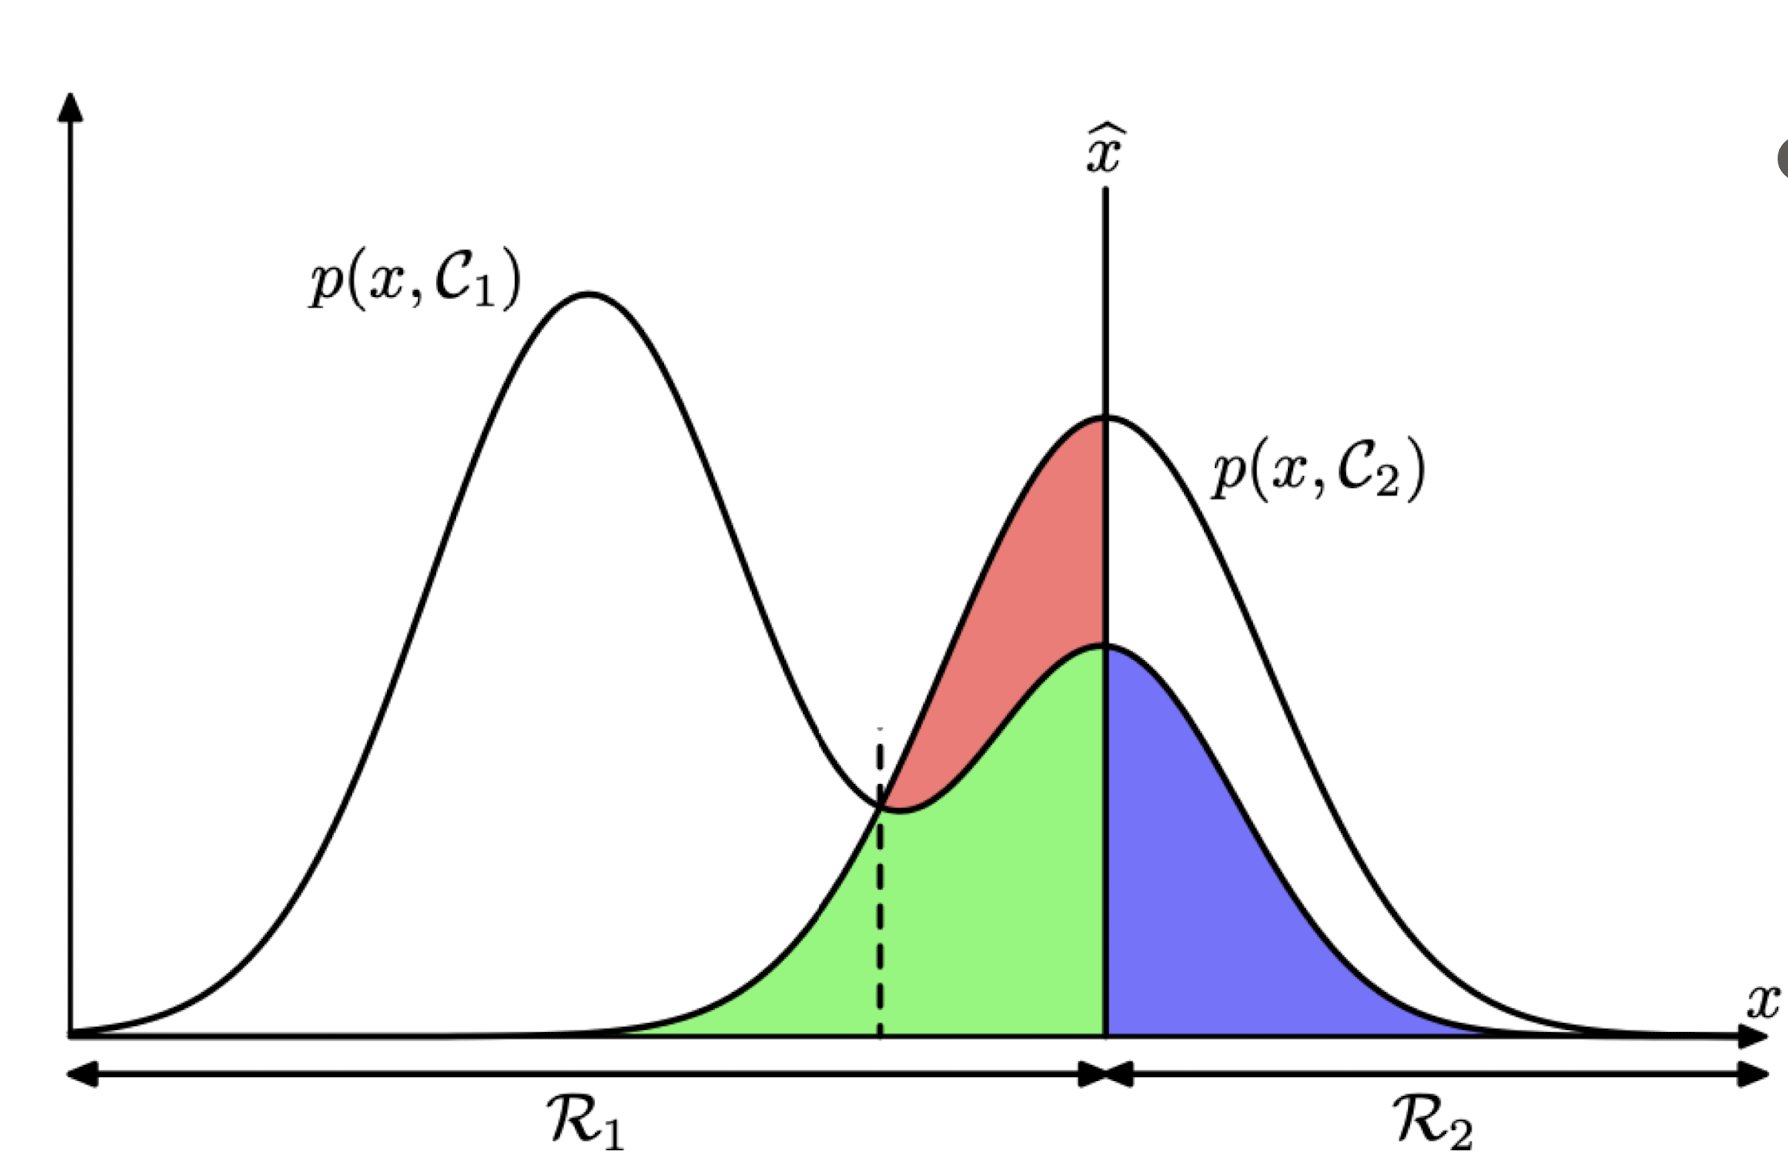
\includegraphics[width=.7\linewidth]{codes/figures/section1/figure_1_1.png}
    \caption{Misclassification Rate}
    \label{fig:my_label}
\end{figure}
\begin{enumerate}
    \item \textbf{RedGreen regions}: inputs that belong to $\mathcal{C}_2$ but assigns to $\mathcal{R}_1$ as they are under $ p\left(x, \mathcal{C}_{2}\right)$.
    \item \textbf{Blue regions}: inputs that belong to $\mathcal{C}_1$ but assigns to $\mathcal{R}_2$ as they are under $ p\left(x, \mathcal{C}_{1}\right)$
    \item Therefore, for any data \textbf{x}, if $ p\left(x, \mathcal{C}_{1}\right)>p\left(x, \mathcal{C}_{2}\right)$, then we assign this point to $\mathcal{C}_1$, vice-versa. Therefore, $\mathcal{R}=\{x:\:p\left(x, \mathcal{C}_{1}\right)>p\left(x, \mathcal{C}_{2}\right)\}$
\end{enumerate}
We want to minimize the misclassification error rate $\Rightarrow$ minimize the \textbf{loss}
\subsection*{Loss Function} 
\textbf{Loss function} measures the loss incurred by taking of any available decisions. 
\subsubsection*{For discrete case}
we denote $L_{ij}$ as the $(k,\:j)$ element of the loss matrix. We want to minimize the expected loss\\
Therefore:
\begin{align*}
\mathbb{E}[L] & =\sum_k \sum_j \int_{\mathcal{R}_j} L_{k j} p\left(x, \mathcal{C}_k\right) d x\\
& =\sum_j \int_{\mathcal{R}_j} \sum_k L_{k j} p\left(x, \mathcal{C}_k\right) d x
\end{align*}
Define $g_j(x)=\sum_k L_{k j} p\left(x, \mathcal{C}_k\right)$. Notice that $g_j(x) \geq 0$ and
$$\mathbb{E}[L]=\sum_j \int_{\mathcal{R}_j} g_j(x) d x$$
Thus, minimizing $\mathbb{E}[L]$ is equivalent to choosing
\begin{align}
    \mathcal{R}_j&=\left\{x: g_j(x)<g_i(x) \text { for all } i \neq j\right\}\\
    \Rightarrow \mathcal{R}_j &=\left\{x: \sum_k L_{k j} p\left(\mathcal{C}_k \mid x\right)<\sum_k L_{k i} p\left(\mathcal{C}_k \mid x\right) \text { for all } i \neq j\right\}
\end{align}
\subsubsection*{For regression}
\begin{itemize}
    \item Consider the input/target $(x,\:t)$, where $t$ is continuous and the joint density is $p(x,\:t)$
    \item The regression function is $y(t)$
    \item The loss function is $L(y(x),\:t)=(y(x)-t)^2$
\end{itemize}
Therefore the expected loss will be:
\begin{align*}
\mathbb{E}[L]&=\iint L(y(x), t) p(x, t) d x d t\\
&=\iint(y(x)-\mathbb{E}[t \mid x])^2 p(x, t) d x d t+\iint(\mathbb{E}[t \mid x]-t)^2 p(x, t) d x dt
\end{align*}
Full derivations \hyperref[derivations-1]{here}\\
The second term is the conditional variance of $t|x$ and does not depend on $y(x)$ and hence the expected loss is minimized when $y(x)=\mathbb{E}[t|x]$. Therefore, we can see that the loss function will change the decision rule significantly; however, we can always reject the option or not making a decision.
